\documentclass[English,c,% 't' (resp. 'c') places text vertically at top/center of each slide
% PDF settings
hyperref={%
  pdftitle={Java Inheritance/Interfaces},%
  pdfauthor={Muller, Gravier, Laforest, Subercaze},%
  pdfsubject={Java Inheritance/Interfaces},%
  pdfkeywords={Inheritance, Interface, Java},%
  colorlinks=true,%
  urlcolor=blue,%
  linkcolor=%
},%
% To load many pre-defined color names
xcolor={pdftex,svgnames} % dvipsnames, dvipsnames*, svgnames, svgnames*, x11names,
]{beamer}

\usetheme{Copenhagen}
% \setbeamertemplate{footline}[page number]
% \setbeamertemplate{frametitle}[default][center]
% To remove the navigation symbols from the bottom of slides:

% Remove navigation bar
\setbeamertemplate{navigation symbols}{}
% Remove outline at top
\setbeamertemplate{headline}{}

% Put text more on top of each slide for all slides
\addtobeamertemplate{frametitle}{}{\vspace*{-.7em}}

% Correct French/English indentation and splitting of words
\usepackage{babel}

% Correct management of accentuated chars in input file
\usepackage[utf8]{inputenc}

% Correct font for the generation of docs with accentuated chars
\usepackage[T1]{fontenc}      % Can handle hyphenation of words with accented characters
%% \usepackage[OT1]{fontenc}   % Might generated bad looking PDFs

% Insertion of images generated by external tools
\usepackage{graphicx}
% To generate pretty & scalable images directly in LaTeX
\usepackage{tikz}

% To print numbers correctly
\usepackage{numprint}

% To print numbers correctly
\usepackage{ulem}

\usepackage[absolute,overlay]{textpos}

\usepackage{fourier}

\setbeamercovered{transparent}
\setbeamercovered{invisible}

\AtBeginSection[]
{
  \begin{frame}
    \frametitle{Plan}
    \tableofcontents[currentsection]
  \end{frame}
}

\usepackage{url,manfnt}


% To be able to insert code listing
\usepackage{listings}

\definecolor{dkgreen}{rgb}{0,0.6,0}
\definecolor{gray}{rgb}{0.5,0.5,0.5}
\definecolor{mauve}{rgb}{0.58,0,0.82}

\lstset{frame=none,
  language=Java,
  aboveskip=1mm,
  belowskip=1mm,
  showstringspaces=false,
  columns=flexible,
  basicstyle={\tiny \ttfamily},
  numbers=left,
  numberstyle=\tiny\color{gray},
  keywordstyle=\color{blue},
  commentstyle=\color{dkgreen},
  stringstyle=\color{mauve},
  breaklines=true,
  breakatwhitespace=true,
  tabsize=2
}
\definecolor{algoTitle}{rgb}{0.84,0.83,0.94}

\usepackage{caption}
\DeclareCaptionFont{white}{\color{white}}
\DeclareCaptionFormat{listing}{\colorbox{algoTitle}{\parbox{\textwidth}{\bfseries #1#2 #3}}}
\captionsetup[lstlisting]{format=listing,labelfont=white,textfont=white}

\title[Java Interface]{Inheritance \& Interfaces in Java}
\logo{
\includegraphics[width=1cm]{images00/logo_tse.png}}
\author[Guillaume MULLER]{
  Guillaume \textsc{Muller}\\
  {\scriptsize \textit{based on work from:} \\
    Ch. \textsc{Gravier}, F. \textsc{Laforest}, J. \textsc{Subercaze}}
}
\institute[TSE/UJM]{
  Télécom Saint-\'{E}tienne\\
  \medskip
  {\url{{pénom.nom}@univ-st-etienne.fr}}
}
\date[09/14/2020]{14~September~2020}

\begin{document}

%%%%%%%%%%%%%%%%%%%%%%%%%%%%%%%%%%%%%%%%%%%%%%%%%%%%%%%%%%%%%%%%%%%%%%
\begin{frame}
  \maketitle
\end{frame}

%%%%%%%%%%%%%%%%%%%%%%%%%%%%%%%%%%%%%%%%%%%%%%%%%%%%%%%%%%%%%%%%%%%%%%
\section{Inheritance}

%%%%%%%%%%%%%%%%%%%%%%%%%%%%%%%%%%%%%%%%%%%%%%%%%%%%%%%%%%%%%%%%%%%%%%
\begin{frame}[fragile]{Declare a Class}
  \vspace{-1em}
  \begin{lstlisting}[escapechar=\%,label=expers,caption=Person.java,basicstyle=\scriptsize]
    public class Person {
      // Attributes
      private String lastName;
      private String firstName;
      // Methods (Constructor)
      public Person (String n, String p) {
        lastName=n;
        firstName=p;
      }
      public void display() {
        System.out.println("First Name: "+firstName+", Last Name: "+lastName);
      }
      public String getName() {
        return name;
      }
    }
  \end{lstlisting}
\end{frame}


%%%%%%%%%%%%%%%%%%%%%%%%%%%%%%%%%%%%%%%%%%%%%%%%%%%%%%%%%%%%%%%%%%%%%%
\begin{frame}[fragile]{Inheritance -- 1}
  \vspace{-1em}
  \begin{lstlisting}[escapechar=\%,label=exelv,caption=Student.java,basicstyle=\scriptsize]
    public class Student extends Person {
      // Attributes
      private int year;
      // Methods (Constructor)
      public Student(String n, String p, int a) {
        super(n,p);
        year=a;
      }
      @Override
      public void display() {
        System.out.println("Name: "+firstName+" "+lastName+" ("+year+")");
      }
    }
  \end{lstlisting}
\end{frame}


%%%%%%%%%%%%%%%%%%%%%%%%%%%%%%%%%%%%%%%%%%%%%%%%%%%%%%%%%%%%%%%%%%%%%%
\begin{frame}{Inheritance -- 2}
  \begin{itemize}
    \item Problem:\\
    Parent \& Child classes are \textbf{tightly coupled} $\Rightarrow$ low reusability
    \bigskip
    \item To prevent too much coupling, Java:
    \begin{itemize}
      \item Does \textbf{not} allow multiple inheritance,
      \item Proposes the concept of \texttt{interfaces}.
    \end{itemize}
  \end{itemize}
\end{frame}

%%%%%%%%%%%%%%%%%%%%%%%%%%%%%%%%%%%%%%%%%%%%%%%%%%%%%%%%%%%%%%%%%%%%%%
\begin{frame}{Single Inheritance}

  \begin{itemize}
    \item In Java it is \textbf{NOT} possible to inherit from multiple classes
    \sout{\texttt{public class MyClass extends Class1, Class2}} \\
    \sout{\texttt{public class MyClass extends Class1, extends Class2}}
    \item Solves many problems at compilation time $\Rightarrow$ speed
    \item Does not reduces expressivity
    \bigskip
    \item $\Rightarrow$ \texttt{interfaces}
  \end{itemize}
\end{frame}


\section{Interfaces}

  %%%%%%%%%%%%%%%%%%%%%%%%%%%%%%%%%%%%%%%%%%%%%%%%%%%%%%%%%%%%%%%%%%%%%%
  \begin{frame}{Interfaces}
    \begin{columns}[t]
      \begin{column}{.55\linewidth}
        \begin{block}{Interfaces in Java}
          An interface defines a behaviour (method prototypes) that must be
          implemented by classes that realize it.
        \end{block}
      \end{column}

      \begin{column}{.40\linewidth}
        \begin{block}{}
          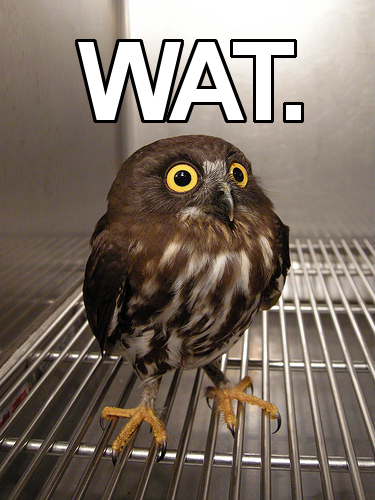
\includegraphics[height=0.6\textheight]{./images01/wat.png}
        \end{block}
      \end{column}
    \end{columns}

  \end{frame}


  %%%%%%%%%%%%%%%%%%%%%%%%%%%%%%%%%%%%%%%%%%%%%%%%%%%%%%%%%%%%%%%%%%%%%%
  \begin{frame}{Interfaces}
    \begin{itemize}
      \item \textbf{Interfaces} list \textbf{methods} common to all the classes that will implementing it;
      \item Inheritance is reserved for when necessary (ex: a Student \textbf{is a} Person);
      \item Interfaces are \textbf{contracts} that the implementing classes must follow;
      \item Interface do \textbf{NOT} detail the \textbf{implementation} of these methods (i.e. all methods are abstract!)\footnote{This changed in Java~8!};
      \item When a class implements an interface, one can be \textbf{certain} that the methods declared in the interface are present.
    \end{itemize}
  \end{frame}




  %%%%%%%%%%%%%%%%%%%%%%%%%%%%%%%%%%%%%%%%%%%%%%%%%%%%%%%%%%%%%%%%%%%%%%
  \begin{frame}[fragile]{Interface: Example -- 1\footnote{\url{http://docs.oracle.com/javase/tutorial/java/concepts/interface.html}}}
    \vspace{-1em}
    \begin{lstlisting}[escapechar=\%,label=intex,caption=Bicycle.java,basicstyle=\footnotesize]
      interface Bicycle {
        // Interfaces do not have attributes

        void changeCadence(int newValue); // Wheel revolutions per minute

        void changeGear(int newValue);

        void speedUp(int increment);

        void applyBrakes(int decrement);
      }
    \end{lstlisting}

  \end{frame}


  %%%%%%%%%%%%%%%%%%%%%%%%%%%%%%%%%%%%%%%%%%%%%%%%%%%%%%%%%%%%%%%%%%%%%%
  \begin{frame}[fragile]{Interface: Example -- 2}
    \vspace{-1.2em}
    \begin{lstlisting}[escapechar=\%,label=intex,caption=ACMEBicycle.java,basicstyle=\footnotesize]
      class ACMEBicycle implements Bicycle {
        int cadence = 0; // Class has attributes
        int speed = 0;
        int gear = 1;
        void changeCadence(int newValue) { // Methods ARE implemented
          cadence = newValue;
        }
        void changeGear(int newValue) {
          gear = newValue;
        }
        void speedUp(int increment) {
          speed = speed + increment;
        }
        ...
      }
    \end{lstlisting}
  \end{frame}

\end{document}
